\documentclass[../../thesis.tex]{subfiles}

\begin{document}

Our work, as well as out models can be divided into two stages. Firstly we investigate the effect of non-contrastive SSL on a proven tokenization model, VQVAE \cite{VQVAE}, with the goal of learning more expressive representations. The expressiveness is measured in terms of the models ability to reconstruct unseen data, as well at the performance of learned latent representations on a downstream classification task. The SSL models we consider are, as introduced in section 2 \todo{make hyperlink}, BarlowTwins and VIbCReg.\\\\

Secondly we investigate the effects of SSL-VQ-VAE on prior learning by training a MaskGIT model on top of the tokenization models.\\\\

Additionally we provide ablations investigating robustness to augmentations and the effect of augmentations reconstruction weight. 




\begin{figure}[h]
    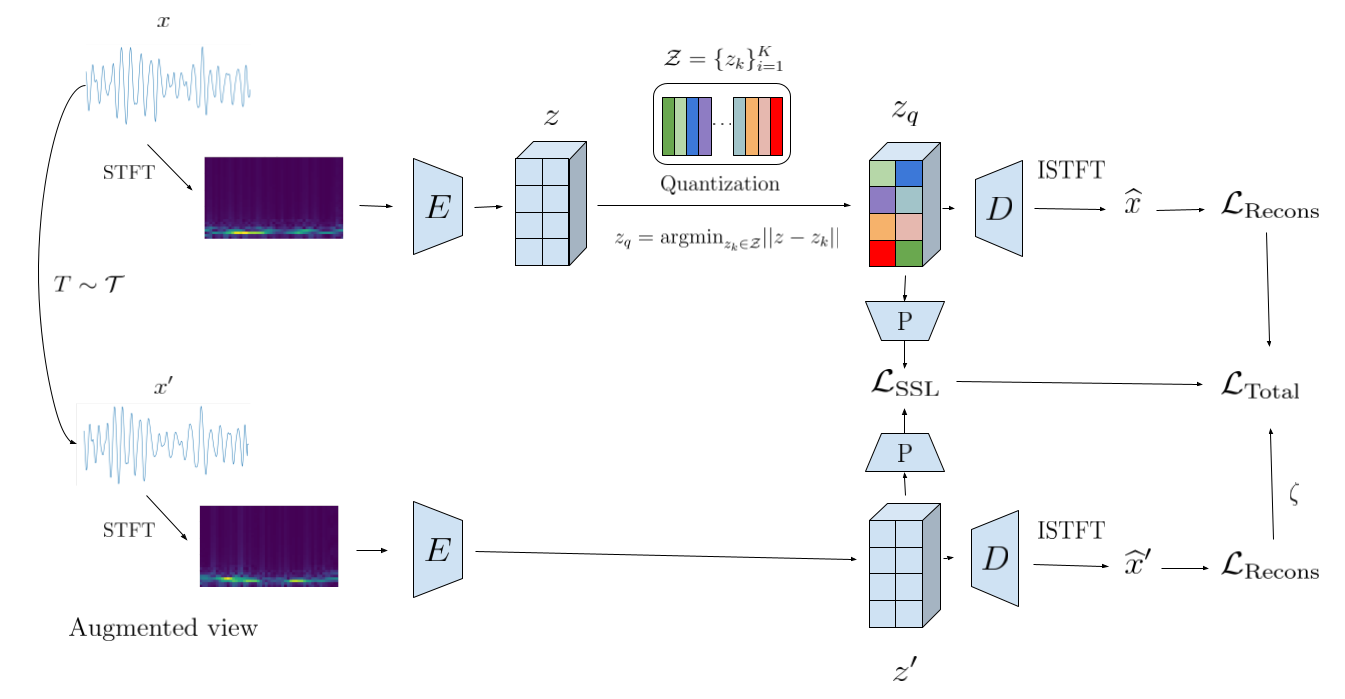
\includegraphics[scale=0.5]{Siam-VQVAE.png}
    \centering    
\end{figure}


\section{Stage 1: Tokenization}


\subsection{VQ-VAE}
The VQ-VAE model is baseline for our experiments.\\

An encoder, decoder, and codebook are to be optimized by compressing the input into discrete latent space, minimizing information loss by comparing input to the output, which ideally are equal. We follow \cite{TimeVQVAE} and augment time-series into time-frquency domain, but leave the high-low frequency split for future work.

\subsubsection{Method}
A schematic overview of the VQ-VAE model is presented in "Figure here"

A time series is first augmented into time-frequency domain using the Short-time Fourier Transform (cite pytorch stft). Then it is encoded into the continuous latent space, and is discretized by the codebook via the argmin process. In the argmin process the continuous token is compared to every discrete token in the codebook, and replaced by the closes discrete token in terms of euclidean distance. Then, the decoder maps the discrete token back to time-frequency domain, before finally being mapped back to time domain using the ISTFT.




\subsubsection{Implementation details}


\subsection{Joint Embedding VQ-VAE}
We have a common framework for the two SSL methods\\\\
We denote the latent variables by $z$ and quantized latent variables $z_q$. All augmented values are denoted by as asterix, i.e $z'$ is a latent variable in the augmented branch. \\\\


The framework is a joint embedding architecture with upper/original branch identical to the VQ-VAE model presented above. The the lowe/augmented branch is identical, except for a lack of quantization layer. 

We compute a SSL loss between derived values of $z_q$ and $z'$. This part is different for VIbCReg and BarlowTwins.  

We compute reconstruction losses $\mathcal{L}_{\text{Rec}}(\hat{x})$ and $\mathcal{L}_{\text{Rec}}'(\hat{x}')$, of both original and augmented view. 
\subsubsection{Method}

\subsubsection{Loss}


\subsubsection{Augmentations}
We used the following collection of augmentation techniques.
\begin{itemize}
    \item Amplitude Resizing
    \item Window Warp
    \item Slice and Shuffle
    \item Gaussian noise
\end{itemize}

\subsubsection{Implementation details}

\subsection{Barlow Twins VQ-VAE}
\subsubsection{Model Architecture}


An encoder, decoder, codebook, and projector are to be optimized. Produce two augmented views of the time-series, augment views into time-frequency domain and encode into latent space. Choose one view for quantization, decoding and comparison to original time series (VQVAE loss). Project both latent embeddings and calculate Barlow loss. Update using both VQVAE and Barlow loss.

A schematic overview of the BT-VQ-VAE model is presented in "Figure here"



\subsection{VIbCReg VQ-VAE}

\subsubsection{Method}

\subsubsection{Implementation details}

\subsubsection{Training}

\section{Stage 2: Prior Learning}

\subsection{MaskGIT}
Regular MaskGIT, token context MaskGIT, learnable codebook MaskGIT

\end{document}